\documentclass[a4paper]{article}
\usepackage{graphicx}
\graphicspath{ {images/} }
\usepackage[english]{babel}
\usepackage[utf8]{inputenc}

\title{Merger Arbitrage Final Report}

\author{Tianyuan Liu, Haoran Wang}

\date{\today}

\begin{document}
\maketitle

\section{Project Introduction}
\label{sec:idea}

One of the classic event-driven investment strategy in finance is called merger arbitrage. Every year, hundreds of public companies in the US are bought out (merged) by other companies. In order to successfully acquire the target company, the acquirer needs to pay a premium, which causes the target company’s share price to jump post-announcement. Since there is uncertainty regarding the success of the acquisition, the target’s post-announcement share price is usually below the acquirer’s offer price. This leads naturally to an investment strategy. If one can accurately predict the success/failure of the merger, one can buy the stocks that will succeed and short the stocks that will fail. Thus, our project goal is to create a model that predicts the success/failure of pending mergers.

\section{Data Description and Cleaning }
\label{sec:data}

Our data set primarily comes from SDC Platinum, a widely used M\&A database in corporate finance. We restrict our data to the years between 1990 and 2016, and only include those that involve a public entity as target. Non-public companies are excluded due to the lack of basic data like purchase price.
\\
\\
Originally, our data has 11678 data points (rows) and 29 features (columns). A shortened summary table of the features and brief description is available at the Appendix. The feature of interest is "Status". Status can take the following values: Completed, Dis Rumor, Intended, Part Comp, Pending, Rumor, Status Unknown, Withdrawn. To simplify our problem, we categorize all values other than "Completed" and "Pending" into "Failed", then we disregard all "Pending" values. \footnote{We tested with only using values "Completed" and "Withdrawn". No significant difference was found} Thus our problem becomes a binary classification problem. We further remove all data points that don't have "Price Per Share", the Acquiror's proposed acquisition price, or with a "Price Per Share" lower than \$1. This is standard practice in the finance literature and justified by the fact that without a known acquisition price, one has no way forming a trading strategy. Stocks that have a share price below \$ 1 usually exhibit funny behaviors and are often excluded from the analyze. We are now left with 8963 data points, which includes 7383 "Completed" and 1580 "Failed".
\\
\\
We then start creating features through feature transformation. Broadly speaking, the new features can be separated into four categories: Valuation, Deal Characteristic, Volatility variables, Time Series variables. A summary of the variables can be found in the appendix. We also made histogram plots of various variables to get a sense of the variables distribution. The features come from a variety of sources, including SDC Platinum, Fama French Database, Compustat and Option Metric.
\\
\\

\begin{center}
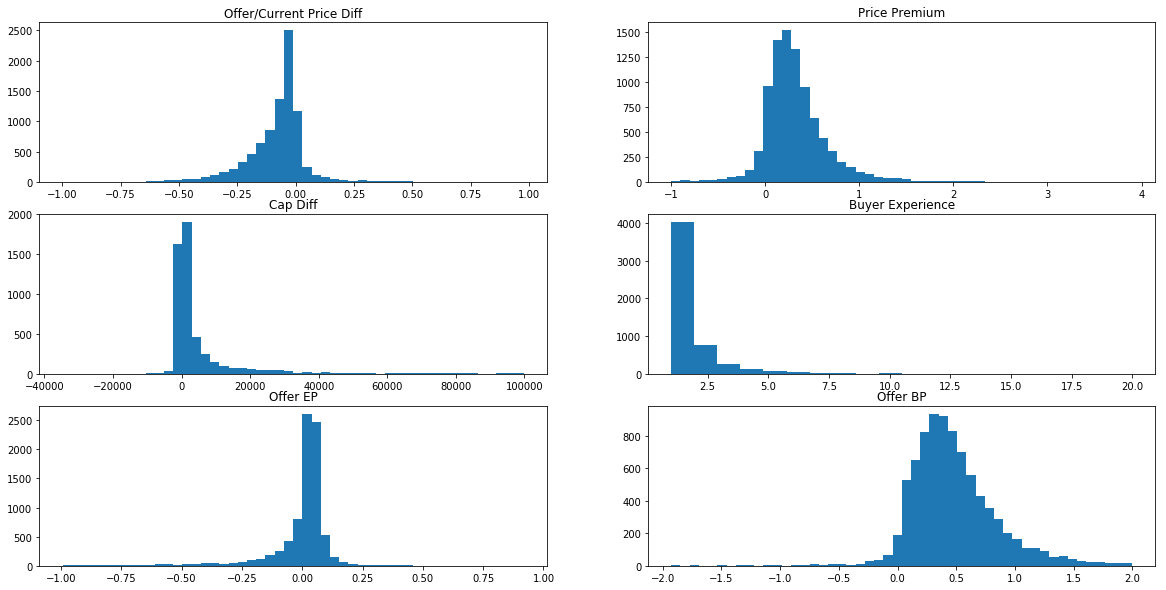
\includegraphics[scale=0.32]{hist.png} 
\end{center}

We note that, given the finance nature of the project, time series variables are inevitable. We've taken special care when dealing with the time series variables to avoid look-ahead bias. The graph below shows the time-varying nature of the success rate. It is possible that additional time-series/macro data can improve the results. This will be left for further research.
\\
\\
For volatility related variables, data came from OptionMetrics, a commonly used database for implied volatility. The volatility variables are mainly implied volatility level and percentage change. Unfortunately, the majority (4/5) of companies didn't have traded options and thus lacked implied volatility data. The volatility variables didn't perform as well as expected, potentially due to the limited number of valid data.
\\
\\

\begin{center}
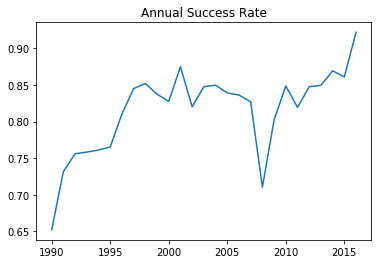
\includegraphics[scale=0.6]{success_rate.png}
\end{center}

Additionally, like all financial data, the data set has many NaN. For example, nearly 1600 data points have a NA for "Percent of Shares Acq.". We tested several different approaches to fill the NA values, including imputation, Principle Component Analysis(PCA) and low rank matrix completion models. For imputation, we tested filling the NAs with mean, median and 0. For low rank matrix completion, we used a Quadratic Loss function with k = 20 \footnote{Since the categorical values don't have missing data, the matrix completion was only performed on the real value data}. We provide a table in the Appendix that summarizes the performance of each model and each filling method. All further analysis below will be based on filling NAs with 0.


\section{Model Selection and Analysis }
\label{sec:model}

Given the time series nature of the data, we couldn't split the training and testing data  randomly. A random split, like what we originally used in our midterm report, will cause look-ahead bias and inflate the results. We split the data on the year 2008. Every deal announced after 2008 are put in the test data set. The training data set consists of 6981 deals, while the test data set contains 2057 deals.
\\
\\
Before fitting the data with a model, we first need to specify what we are trying to outperform. Given the fact that we have more "Completed" than "Failed", we will aim to outperform a strategy that blindly guesses "Completed". The benchmark has a success rate of 83.6\%. This will prove to be a very hard rate to outperform. We try the following models on our data set: Logistic Regression, Decision Tree, Random Forest, Nearest Neighbor.
\\
\\
We now have 73 features in our data set. It is likely that many of the features are redundant. Thus we start our analysis using a logistic regression with L1 penalty. Unfortunately, the logistic model fails to outperform the benchmark; however, as expected, the lasso penalty quickly kills many features. 
\\
\\
We next try a simple decision tree. We provide a illustrative graph below as an example of a possible split. It should be noted that one node only has 1 value, which is a dangerous sign of over fitting. 
\\
\\
\begin{center}
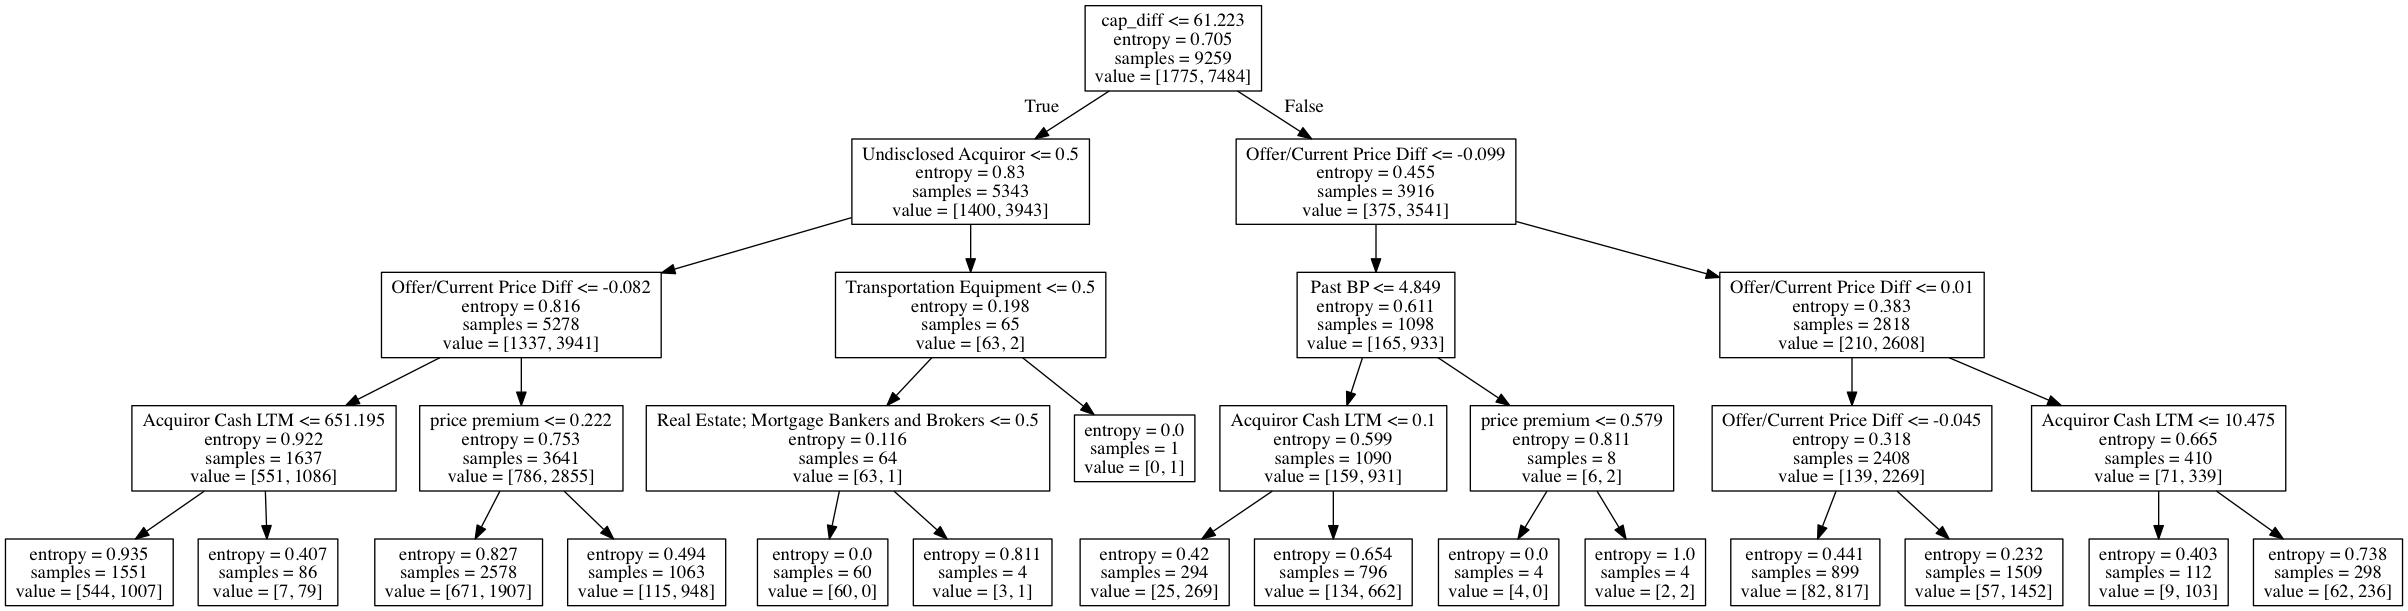
\includegraphics[width=14cm, height=5cm]{tree.png} 

\end{center}

We then try a random forest classifier. Compared to a simple decision tree, a random forest classifier is much less prone to over-fitting. The random forest classifier performs slightly better. After choosing parameters using cross-validation, the model outperforms the benchmark by around 0.2 percent. This out-performance is not significantly different from the benchmark and nearly negligible. The random forest classifier also allows us to calculate the importance of each feature. We provide a bar chart below that shows the top features. Consistent with our intuition, "Offer/Current Price Diff" is the most important feature. We note that the training success rate is particularly high, which might indicate over-fitting. Cross-validation might not be enough, given the high dimensionality.
\\
\\
We also try a nearest neighbor classifier on our data set. The training success rate and testing success rate all under performed the random forest classifier. Given the high noise inherited in the data, the under-performance isn't surprising.
\\
\\

\begin{center}
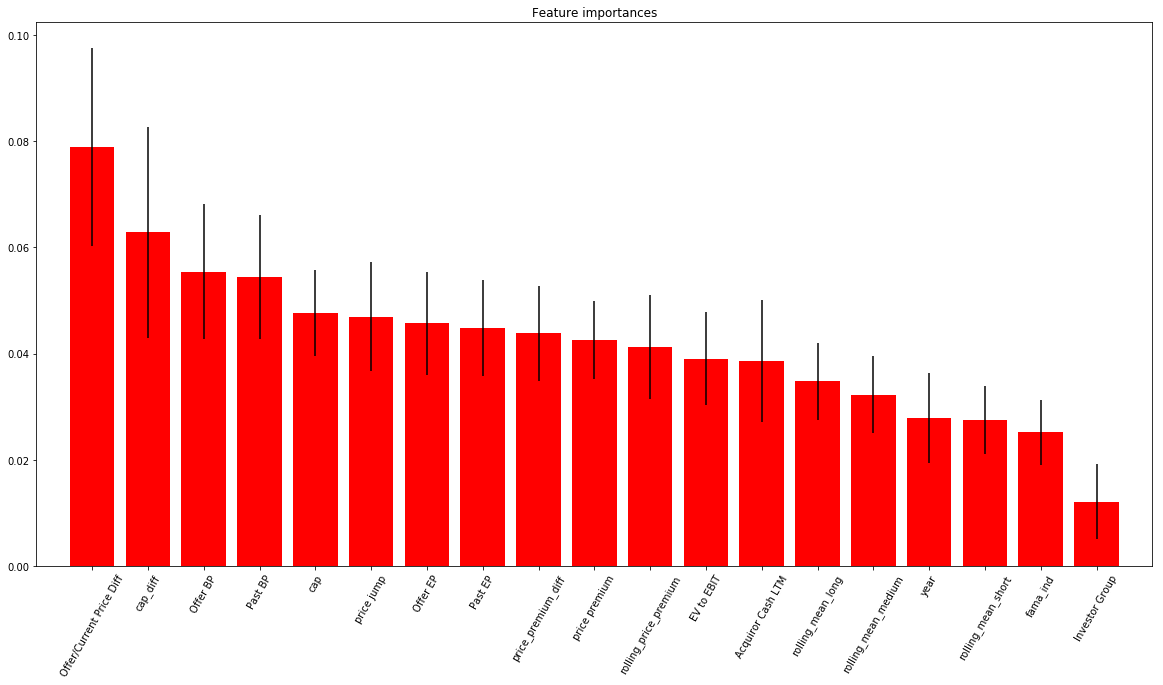
\includegraphics[width=14cm, height=8cm]{Feature_Importance.png} 

\end{center}


\section{Conclusion and Future Steps }
\label{sec:conclusion}

The improvement over the benchmark is quite disappointing. It shows the difficulty of outperforming the market, especially with limited data. The unprecedentedly high success rate in the past decade might have made the benchmark too high to beat. Sentiment data on news report regarding the merger announcement can be potentially very useful, unfortunately also beyond our project's scope. Looking ahead, we still see great potential in the idea, and believe it's worthy of further research. 

\newpage 
\section{Appendix }
\label{sec:tables}

\begin{table}[h]
\caption{Feature Description}
\begin{tabular}{ll}
Date Ann                 & Date of Merger Announcement                                  \\
Status                   & Final status of the deal                                     \\
\% of Shares Acq.        & \% of share the Acquiror aims to acquir                      \\
Price Per Share          & The price per share the Acquiror offers                      \\
Shares Out Actual        & Target's number of shares outstanding                        \\
Acquiror Cash LTM        & Acquiror's cash amount                                       \\
EV to EBIT               & Enterprise Value over Earning Before Interest and Tax        \\
Democrat/Republican      & Whether the deal happened during a Democrat presidency       \\
First Time               & Whether this is the first time the Acquiror has done a merger \\
Experienced              & more then 1 less then 20                            \\
nation diff              & Whether target and acquiror are from different nations       \\
industry diff            & Whether target and acquiror are from different industrys     \\
Offer/Current Price Diff & Offer price / price 1 day after announcement                 \\
Price Premium            & Offer price / price 1 day before announcement                \\
cap diff                & Capitalization difference between target and acquiror       \\
rolling mean short               & Success rate in the past 30 days  \\
rolling mean long              & Success rate in the past year                            \\
year              & Year of deal       \\
Target Vol jump 30         & Change of 30 day option implied volatility for target     \\
Acquiror Volatility 14 & 34 day option implied volatility for acquiror              \\
29          & Fama French industry classification - industry 29            
\end{tabular}
\end{table}

\begin{table}[h]
\caption{Summary of Model Results}
\label{my-label}
\begin{tabular}{lll}
\hline
                                            & Train Success & Test Success \\ \hline
Random Forest with Matrix Completion        & 0.952         & 0.836        \\ \hline
Random Forest with 0 as NA                  & 0.974         & 0.838        \\ \hline
Random Forest with Mean as NA               & 0.97          & 0.831        \\ \hline
Random Forest with Median as NA             & 0.961         & 0.834        \\ \hline
Random Forest with PCA decomposition (n=15) & 0.877         & 0.836        \\ \hline
Logistic Regression with 0 as NA            & 0.819         & 0.836        \\ \hline
Nearest Neighbor with 0 as NA               & 0.823         & 0.829        \\ \hline
Decision Tree with 0 as NA                  & 0.822         & 0.831        \\ \hline
Benchmark                                   &               & 0.836       
\end{tabular}
\end{table}

\end{document}
